\documentclass{article}
\usepackage[T1]{fontenc}
\usepackage{lmodern}
\usepackage{graphicx}
\usepackage{amsmath,amssymb}
\usepackage[a4paper,margin=2cm]{geometry}
\usepackage[absolute,overlay]{textpos}
\setlength{\TPHorizModule}{1mm}
\setlength{\TPVertModule}{1mm}
\usepackage[indonesian]{babel}
\usepackage{hyperref}
\setlength{\emergencystretch}{2em}
% unit: Halaman 14

\begin{document}

% === Halaman 14 (llm) ===

\textbf{Enkripsi:}

\[ E_K(P) = (P \oplus K) \ll 1 \]

\vspace{20mm}

Jadi, hasil enkripsi plainteks

\[ 10100010001110101001 \quad (\text{A23A9 dalam notasi HEX}) \]

adalah

\[ 00100011000100100100 \quad (\text{23124 dalam notasi HEX}) \]

% deskripsi: Proses perhitungan XOR antara dua deret biner, pergeseran 1 bit ke kiri, dan konversinya ke notasi hexadecimal.
% bbox normalisasi: [0.3200, 0.2300, 0.7300, 0.5200]
\begin{textblock*}{86.10mm}(67.20mm,68.31mm)
\noindent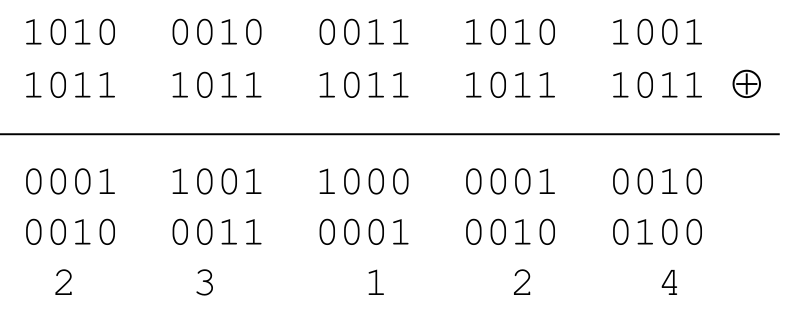
\includegraphics[width=86.10mm,height=86.13mm]{../../images/llm/page_014_img_01.png}%
\end{textblock*}

\end{document}
